\documentclass[11pt]{article}
\usepackage[sc]{mathpazo} %Like Palatino with extensive math support
\usepackage{fullpage}
\usepackage[authoryear,sectionbib,sort]{natbib}
\linespread{1.7}
\usepackage[utf8]{inputenc}

%%%%%%%%%%%%%%%%%%%%%
% LaTeX packages
%%%%%%%%%%%%%%%%%%%%%
% Please be sparing in your use of additional LaTeX packages, and
% upload any required style files to Editorial Manager with the file
% type "LaTeX ancillary files (.sty, .bst)."
\usepackage{amsmath}
%\usepackage{graphicx}
%\graphicspath{ {IMAGES/} }

%%%%%%%%%%%%%%%%%%%%%
% Line numbering
%%%%%%%%%%%%%%%%%%%%%
\usepackage{lineno}
% Please use line numbering with your initial submission and
% subsequent revisions. After acceptance, please comment out 
% the commands \usepackage{lineno}, \linenumbers{} 
% and \modulolinenumbers[3] below.

\title{When predators help prey adapt and persist in a changing environment}

%%%%%%%%%%%%%%%%%%%%%
% Authorship
%%%%%%%%%%%%%%%%%%%%%
% Please remove authorship information while your paper is under review,
% unless you wish to waive your anonymity under double-blind review. 
% Remember to uncomment the information after acceptance.

\author{Matthew M. Osmond$^{1,\ast}$ \\
Sarah P.\ Otto$^{1}$ \\
Christopher A.\ Klausmeier$^{2}$}

\date{}

\begin{document}

\maketitle

\noindent{}1. Biodiversity Research Centre and Department of Zoology; University of British Columbia, Vancouver, BC, Canada;

\noindent{}2. W.K.\ Kellogg Biological Station; Program in Ecology, Evolutionary Biology \& Behavior; and Department of Plant Biology; Michigan State University, Hickory Corners, MI, USA

\noindent{}$\ast$ Corresponding author; e-mail: mmosmond@zoology.ubc.ca.

\bigskip

\textit{Manuscript elements}: Figure~1, figure~2, figure~3, figure~4, figure~5, figure~6,
online appendix~A, and supplementary material.

\bigskip

\textit{Keywords}: Adaptation, evolutionary rescue, extinction, coevolution, quantitative genetics, trophic interactions.

\bigskip

\textit{Manuscript type}: Article. 
% Or e-article, note, e-note, natural history miscellany,
% e-natural history miscellany, comment, reply, symposium, or
% countdown to 150.

\bigskip

\noindent{\footnotesize Prepared using the suggested \LaTeX{} 
template for \textit{Am.\ Nat.}}

\linenumbers{}
\modulolinenumbers[3]

\newpage{}

\section*{Abstract}

To persist in a changing world, populations must adapt. The ability to adapt is influenced by interactions with other species, such as predators. Recent experiments and theory suggest that selective pressures arising from predation may help prey adapt phenotypically to changing environments, but how this influences persistence remains unclear. In particular, it has not yet been shown if predator-induced adaptation can outweigh predator-imposed reductions in population size, allowing prey to persist when they would otherwise go extinct. Here we examine if (and if so, how) predation can enhance the ability of prey to persist in a directionally changing environment. To do so we extend a single-species quantitative-genetics framework that predicts rates of environmental change beyond which populations go extinct. While we assume predation decreases prey density, we find that predators can indeed help prey persist if they sufficiently increase prey adaptedness (decrease phenotypic lag). We show two ways this can occur: 1) the selective push: predators consume maladapted individuals and thus add selection that ``pushes" the mean prey trait toward its optimum, and 2) the evolutionary hydra effect: when predation reduces prey density and thereby increases prey birth rate, allowing more selective events per unit time and effectively reducing generation time. We also discuss how our results apply more broadly, to sources of mortality beyond predation.

\newpage{}

\section*{Introduction}

% The journal does not have numbered sections in the main portion of
% articles. Please refrain from using section references such as
% section~\ref{section:CountingOwlEggs}, and refer to sections by name
% (e.g. section ``Counting Owl Eggs'').

% Please note that we prefer (\citealt{Xiao2015}) to \citealt{Xiao2015},
% since \citealt{} inserts a comma after "et al."

%%GENERAL AREA
Populations are increasingly facing directional environmental shifts caused by climate change and other anthropologic impacts (reviewed in \citealt{Parmesan2003,Davis2005,Parmesan2006,Visser2008,Lavergne2010,Hoffmann2011}).
For example, migrating birds face earlier springs (\citealt{Moller2008}), diapausing insects face later winter onsets (e.g., \citealt{Bradshaw2001}), and ectotherms face warming temperatures (e.g., \citealt{Huey2009,Thomas2012}).
Dispersal and plasticity can help maintain adaptedness and prolong persistence (\citealt{Holt1990,Gienapp2008}), but long-term survival ultimately requires genetic adaptation (\citealt{Visser2008,Gienapp2013}).

The ability of a population to adapt to environmental change commonly depends on interactions with other species (\citealt{Holt1990,Harrington1999,Tylianakis2008,Gilman2010,VanderPutten2010,Lavergne2010,Lawrence2012}).
One ubiquitous interaction is predation, which can impose strong demographic and selective effects
(\citealt{Dawkins1979,Abrams2000b,Reznick2008}). 
Because predators tend to reduce prey population sizes (\citealt{Holt2008b,Salo2010}), thus imposing `demographic costs', they can increase the probability of prey extinction following environmental change (\citealt{Schoener2001}).
However, predators can also induce adaptive phenotypic evolution.
For example, \cite{Tseng2015} have shown that \textit{Daphnia pulex}, which tend to have smaller body sizes in warm water, evolve to smaller sizes and achieve higher population growth rates when reared in warm water with predators than without.
This suggests that predators can sometimes help prey adapt phenotypically in changing environments.
However, increased phenotypic adaptation does not necessarily result in increased persistence.
If predators are to help maintain biodiversity in the face of environmental change it must be shown that predator-induced adaptive phenotypic evolution can outweigh predation's demographic cost and allow prey to persist in environments in which they otherwise could not.
The results have obvious implications for the fate and conservation priority of populations with and without predators (e.g., continental vs.\ island, endemic vs.\ invasive) as well as the conservation practice of removing the predators of threatened populations (\citealt{Reynolds1996,Smith2010}).

%%CURRENTLY HELD VIEWS
There is a small but growing number of theoretical studies on adaptation to gradual, directional environmental change that incorporate interactions between species (\citealt{deMazancourt2008,Jones2008,Johansson2008,Norberg2012,Mellard2015}).
Only two of these studies assessed predator-prey interactions.
\cite{Jones2008} used simulations to study, among other things, a predator-prey system where the predator trait evolves to match the prey trait and the prey trait evolves both to match the changing environmental optimum and escape the predator. 
His main finding was that predation can sometimes increase the persistence time of the prey, presumably when the predator removes prey that are maladapted to the abiotic environment.
\cite{Mellard2015} studied an explicit resource-plant-herbivore trophic chain using a primarily numerical approach to ask how the addition of an herbivore affects plant persistence in a warming environment.
They analytically clarified the conditions required for the predator to hasten prey evolution but found in simulations that, regardless of the effect on evolutionary rates, herbivory almost never aided plant persistence. 
In addition, \cite{Northfield2013}, who did not explicitly model a gradually changing environment, analytically demonstrated that `conflicting' interactions, such as predation, tended to dampen the direct effect of small environmental changes on the equilibrium densities of interacting species, potentially facilitating persistence.
In their model, coevolution facilitates persistence through negative feedback loops. 
For example, as the predator nears extinction the prey invests less in defence, making it easier for the predator to consume prey and rebound in abundance.
Thus, up to this point, while it is clear that predators can theoretically help prey adapt in changing environments, the effect of predators on prey persistence remains unresolved.

%%APPROACH
Here we clarify the effect of predators on the ability of prey to persist in a gradually changing environment within a well established quantitative-genetic framework  (\citealt{Pease1989,Lynch1991,Lynch1993,Burger1995,Burger1997,Lande1996,Chevin2010}), which can be applied to both laboratory (\citealt{Willi2009}) and wild (\citealt{Gienapp2013}) populations.
The framework allows analytical predictions of population densities and mean trait values, as well as the critical rate of environmental change, defined as the minimum rate of environmental change that causes an equilibrium population size of zero.
Under this framework, predators affect prey persistence if they alter the prey's critical rate of environmental change.

%%IMPORTANT FINDING
While there are many ways for predators to hinder prey persistence (most obviously by reducing prey population size), we find that predators can help prey persist when 1) predators prefer maladapted prey and thus push the mean prey trait closer to its moving optimum (`selective push') and when 2) the potentially non-selective mortality induced by predators increases prey birth rates and thus increases the rate of selective events, accelerating prey evolution (`evolutionary hydra effect').

%%%%%%%%%%%%%%%%%%%%%%%%%%%%%%%%%%%%%%%%%%%%%%%%
\section*{Methods and Results}
%%%%%%%%%%%%%%%%%%%%%%%%%%%%%%%%%%%%%%%%%%%%%%%%

%%%%%%%%%%%%%%%%%%%%%%%%%%%%%%%%%%%%%%%%%%%%%%%%
\subsection*{A general model of generalist predation}
%%%%%%%%%%%%%%%%%%%%%%%%%%%%%%%%%%%%%%%%%%%%%%%%

Let prey individuals with trait value $z$, in a prey population of density $N$, be born at a per capita rate of $b(z,N)$ and die with predator-independent per capita mortality rate $m(z,N)$. 
Additionally, let a population of predators kill prey individuals at a per prey rate of $k f(z,N)$, where $k$ is the overall predation intensity and $f$ includes the potential dependence on prey trait value, which describes direct selective effects (e.g., increased consumption of slow, large, or maladapted individuals), as well as the potential dependence of predation on prey density, which allows, for example, a type-II or type-III functional response.
We do not explicitly model predator density and trait values here (but see the ``Specialist predation" section). 
Instead, we assume the predator is a generalist that consumes a sufficient number of other prey species such that its density and trait values are relatively constant and the predation rate depends only on the density and trait values of the focal prey.
Alternatively, constant predator trait values and density could result from the predator having a much longer generation time than the prey or from predator migration from nearby habitats.
For example, with a type-II functional response with handling time $h$ and attack rate $a(z)$ we have $k f(z,N) = a(z) [1 + h a(z) N]^{-1} P$, where predator density $P$ is approximately constant over the timescale of interest.
Although we wish to interpret $k f(z,N)$ as generalist predation here, it could arise from any source of mortality whose per capita rate does not vary too much in time with factors other than prey trait value and population density.
Under these conditions the rate of change in prey density is approximately
\begin{equation}\label{dPdtGen}
\begin{aligned}
\frac{\mathrm{d}N}{\mathrm{d}t} &= N \int_{-\infty}^{\infty} \left[ b(z,N) - m(z,N) - k f(z,N) \right] p(z) \mathrm{d}z \\
&= N \left[ \bar{b}(\bar{z},N) - \bar{m}(\bar{z},N) - k \bar{f}(\bar{z},N) \right],
\end{aligned}
\end{equation}
where $p(z)$ is the probability distribution of trait values in the prey population, $\bar{b}$, $\bar{m}$, and $k\bar{f}$ are the population mean per capita birth, non-predator mortality, and predation rates, respectively, and $\bar{z}$ is the population mean trait value.

When phenotypic variance is small the rate of evolution in the mean trait value is roughly (\citealt{Lande1976}) 
\begin{equation}\label{dbarzdtGen}
\begin{aligned}
\frac{\mathrm{d}\bar{z}}{\mathrm{d}t} &= V_A \frac{\partial}{\partial\bar{z}} \left( \frac{1}{N} \frac{\mathrm{d}N}{\mathrm{d}t} \right)\\
&\propto \frac{\partial\bar{b}}{\partial\bar{z}} - \frac{\partial\bar{m}}{\partial\bar{z}} - k\frac{\partial\bar{f}}{\partial\bar{z}},
\end{aligned}
\end{equation}
where $V_A > 0$ is the additive genetic variance, which determines the strength of the response to selection.
Predators could potentially affect prey adaptation by influencing prey variance, $V_A$, but here we simplify the dynamics and assume the variance is constant and independent of predation.
In the examples that follow, a constant variance results from assuming that offspring trait values are near the mean of their parents.
This causes an equilibrium to be reached between the variance introduced by segregation and recombination and the variance lost through random mating (see supplementary \texttt{Mathematica} file for details). 

We now consider prey evolution in a changing environment.
Let there be some `optimal' trait value, $\theta$, that maximizes prey growth rate at a given density in the absence of predators (i.e., $z=\theta$ maximizes $b-m$ at a given $N$).
We assume that the environmental change causes this optimum to increase linearly at rate $\delta$. 
If the prey persists the mean prey trait will evolve to track the optimum, eventually settling into a steady-state lag (\textit{sensu} \citealt{Lynch1991}) with the mean trait value typically trailing the optimum by a constant amount.
A steady-state is achieved when prey density is constant in time (Equation \ref{dPdtGen} is zero) and the rate of evolution (Equation \ref{dbarzdtGen}) is equal to the rate of change in the environment, $\delta$.
Assuming a stable steady-state exists we can solve for equilibrium population density ($\hat{N}$) and the corresponding steady-state lag [$\hat{L} = \lim_{t\rightarrow\infty}L = \lim_{t\rightarrow\infty}(\theta - \bar{z})$].
The minimum rate of change in the optimal trait value that causes extinction at this steady-state lag ($\hat{N}=0$) gives the critical rate of environmental change, $\delta_c$ (\textit{sensu} \citealt{Lynch1991}).
This is the slowest rate of environmental change that deterministically causes the prey to go extinct (unless the steady-state first loses stability, see discussion in Generalist Example 2).

What we ultimately want to know is how increased predation intensity affects prey persistence, $\mathrm{d}\delta_c/\mathrm{d} k$.
This will depend on how predators affect prey adaptation, which we turn to first.
We begin with a very general description and follow this with concrete examples, where we choose specific functional forms for the terms in Equation \eqref{dPdtGen}.

%%%%%%%%%%%%%%%%%%%%%%%%%%%%%%%%%%%%%%%%%%%%%%%%
\subsubsection*{Effect of predators on prey adaptation}

We begin with the reasonable assumption that increasing predation intensity decreases prey density at a given mean lag, $\partial N/\partial k < 0$ (see \citealt{Abrams2009b} for exceptions). 
Without loss of generality, we specify the direction in which the trait is measured such that the mean prey trait value lags behind the optimum.
Then a small increase in the mean trait value would increase the mean prey growth rate in the absence of the predator, $\partial(\bar{b}-\bar{m})/\partial \bar{z} > 0$.
We say that predation selects in the same direction as the environment when increasing mean prey trait value decreases predation as well as increases the mean prey growth rate in the absence of predators, that is, when $\partial \bar{f}/\partial\bar{z}$ and $\partial (\bar{b} - \bar{m})/\partial\bar{z}$ have opposite signs.

Despite its negative effect on prey density, predation could help the prey persist if it helps the prey adapt, that is, if increasing the predation intensity increases the rate at which prey evolve. 
Mathematically, predators help prey adapt when
\begin{equation}\label{dcdevo}
\begin{aligned}
0<&\frac{\mathrm{d}}{\mathrm{d}k} \frac{\mathrm{d}\bar{z}}{\mathrm{d}t}\\
0<& \frac{\partial}{\partial N} \left( \frac{\partial \bar{b}}{\partial\bar{z}} \right) \frac{\partial N}{\partial k} - \frac{\partial}{\partial N} \left( \frac{\partial\bar{m}}{\partial\bar{z}} \right) \frac{\partial N}{\partial k} - k \frac{\partial }{\partial N} \left( \frac{\partial\bar{f}}{\partial\bar{z}} \right) \frac{\partial N}{\partial k} - \frac{\partial \bar{f}}{\partial\bar{z}}  .
\end{aligned}
\end{equation}
Thus, to know if increasing predation intensity could speed up the rate of prey evolution we need to know the likely signs of the terms on the right hand side of Equation \eqref{dcdevo}.

Most intuitively, the last term in Equation \eqref{dcdevo} shows that when predators select in the same direction as the environment (here $\partial \bar{f}/\partial \bar{z}<0$) -- what we call a `selective push' -- increased predation intensity will help the prey adapt directly through selection regardless of whether the predation rate is density-dependent (Figure \ref{Diagram}).
Of course, selection from the predator that opposes selection from the environment (a `selective pull`, here $\partial \bar{f}/\partial \bar{z}>0$) will hinder prey adaptation.

Even without direct selection via predation ($\partial \bar{f} / \partial \bar{z}=0$), predators can facilitate adaptation by altering prey demography.
Negative density-dependence causes birth rates to decline with population density, $\partial \bar{b}/\partial N < 0$. 
Thus we may expect that the mean per capita birth rate will increase less with mean trait value at higher densities, $\partial (\partial\bar{b}/\partial\bar{z}) / \partial N< 0$.
Therefore, with negative density-dependent population growth and our initial assumption that predation decreases prey density ($\partial N/\partial k<0$), increasing predation intensity can help prey adapt when selection and density-dependence act on births (first term in Equation \ref{dcdevo}). 
Essentially, the predator (or any other form of non-selective mortality) depresses prey density, which elevates prey birth rates, increasing the expected number of selective events in a given time and thus accelerating the rate of evolution in a changing environment (Figure \ref{Diagram}).
We call this phenomenon the `evolutionary hydra effect' (after the non-evolutionary `hydra effect' described by \citealt{Abrams2009b}), referring to the ability of the mythical monster to regrow two heads for every one severed by Heracles.
In our case, due to selection, the heads that grow back tend to be better adapted than the one that was severed.
The evolutionary hydra effect can occur whenever generation times can be decreased, allowing more opportunity for selection per unit time.
This applies to univoltine species with overlapping generations (e.g., many temperate bird species), whenever the average age of one's parent is decreased by mortality.
Generation times cannot, however, be decreased in univoltine species with non-overlapping generations, where generation time is fixed (e.g., annual plants; see supplementary \texttt{Mathematica} file for discrete time models with overlapping and non-overlapping generations). 

The opposite is true for per capita death rates; with negative density-dependence, increasing density increases death rates, $\partial \bar{m}/\partial N > 0$, making it likely that death rates decrease more with increases in trait value at high densities, $\partial (\partial \bar{m}/\partial \bar{z}) /\partial N < 0$.
That is, the opportunity for selection via natural mortality is likely to be stronger at larger population sizes (in the absence of predators) than at smaller ones (with predators).
Thus, selection and negative density-dependence acting on prey mortality (along with $dN/dk$) means that predation likely reduces the ability of prey to adapt (the second term in Equation \ref{dcdevo} is likely negative). 
However, with positive density-dependence (e.g., when the population size is very small and there are Allee effects) the situation is reversed; increased predation rates could then help the prey adapt when selection and density-dependence both act on death, rather than birth.

Assuming negative density-dependence again, predation can also help the prey adapt if $-\partial (\partial\bar{f}/\partial\bar{z}) / \partial N < 0$ (third term in Equation \ref{dcdevo}).
This is most likely when per capita predation rates weaken as the population size grows ($\partial \bar{f}/\partial N<0$) so that predation is more effective -- and more selective -- when predation has depressed prey densities.
Whether this occurs depends on the nature of the functional response.
A type-I functional response implies that density has no effect on per capita predation rates ($\partial \bar{f}/\partial N = 0$), a type-II functional response implies that density has a negative effect on per capita predation rates ($\partial \bar{f}/\partial N < 0$), while a type-III functional response implies that density has a positive effect on per capita predation rates at low densities ($\partial \bar{f} /\partial N > 0$) and a negative effect on per capita predation rates at high densities ($\partial \bar{f} / \partial N < 0$).
It is therefore possible for increasing predation intensity to aid adaptation indirectly through changes in density (as in the evolutionary hydra effect described above) even if prey birth and natural mortality are not selective (first two terms in Equation \ref{dcdevo} are zero) but predation is ($\partial \bar{f}/\partial \bar{z}\neq0$).
This would occur, for example, with a type-II functional response and predation that selects in the same direction as the environment.
In this case, the decreased prey density resulting from increased predation intensity causes an increase in the per capita rate of predation, and since predation selects in the same direction as the environment it accelerates the evolution of the mean prey trait value towards the optimum (i.e., the evolutionary hydra effect enhances the selective push).

%%%%%%%%%%%%%%%%%%%%%%%%%%%%%%%%%%%%%%%%%%%%%%%%
\subsubsection*{Effect of predators on prey persistence}

While considering the form of Equation \eqref{dcdevo} provides insight into when predation can help prey adapt (decreased phenotypic lag), satisfying this condition does not necessarily mean that predation will help prey \textit{persist} (maintain positive population density) in a more rapidly changing environment.  
Because predation reduces prey density, it can lower the critical rate of environmental change, $\delta_c$, even if the prey are more adapted.  

From Equation \eqref{dbarzdtGen}, we can write the critical rate of environmental change as
\begin{equation}
\delta_c = V_A \frac{\partial g(\bar{z},k)}{\partial \bar{z}}\Big|_{\bar{z}=\bar{z}_c(k)},
\end{equation}	
where $g(\bar{z},k) = \bar{b}(0,\bar{z})-\bar{m}(0,\bar{z})-k\bar{f}(0,\bar{z})$ is the per capita growth rate when rare (invasion fitness) and $\bar{z}_c(k)$ is the mean trait value that causes equilibrium population size to be zero (critical trait value).
Letting $h(\bar{z}_c(k),k) = \partial g(\bar{z},k) / \partial \bar{z}\big|_{\bar{z}=\bar{z}_c(k)}$ be the selection gradient at the critical rate, we can take the derivative with respect to predation intensity on both sides, showing that predation increases the critical rate when
\begin{equation}\label{dkcdc}
\begin{aligned}
0 &< \frac{\mathrm{d} \delta_c}{\mathrm{d} k} = V_A \left[ \frac{\partial h}{\partial k} + \frac{\partial h}{\partial \bar{z}_c} \frac{\partial \bar{z}_c}{\partial k} \right] \\
0 &< V_A \left[ \frac{\partial^2 g}{\partial \bar{z}\partial k } + \frac{\partial^2 g}{\partial \bar{z}^2} \frac{\partial \bar{z}_c}{\partial k} \right]_{\bar{z}=\bar{z}_c(k)} ,
\end{aligned}
\end{equation}	
Restricting ourselves to cases where extinction occurs because equilibrium population density goes to zero (as opposed to an unstable steady-state), predation helps persistence when it helps adaptation by bringing the trait closer to the optimum (Equation \ref{dcdevo} is satisfied) and increases the critical rate of environmental change (Equation \ref{dkcdc} is satisfied). 

The first term inside the brackets of Equation \eqref{dkcdc}  is a mixed derivative that describes the impact of selective predation on persistence.
It is negative when there is a selective pull, positive when there is a selective push, and zero otherwise.
The second term is comprised of two derivatives.
One of these is a second derivative that describes how the shape of invasion fitness changes with mean trait value.
It is zero when invasion fitness depends linearly on trait value, negative when invasion fitness increases slower with trait value at trait values closer to the optimum (concave down), and positive when invasion fitness increases faster with trait value closer to the optimum (concave up).
The second part of the second term describes how the critical trait value depends on predation intensity. 
Since predation is assumed to lower per capita growth rate, the critical trait value will increase with increases in predation intensity, and thus this derivative is positive (i.e., a prey population on the brink of extinction needs to become better adapted to the abiotic environment if it is to persist with more predation).
We can therefore reason that in the absence of selective predation the evolutionary hydra effect will help persistence if and only if invasion fitness is concave up at the critical trait value.
For example, if selection occurs only through births, the evolutionary hydra effect cannot help persistence if birth rate is a quadratic function of phenotype (concave down for all trait values), but it can if birth rate is a Gaussian function (concave up for critical trait values that are sufficiently far from the optimum). 
In other words, small decreases in lag at the persistence boundary must cause large enough increases in invasion fitness for the evolutionary hydra effect to help persistence.
Recall too that Equation \eqref{dcdevo} must also be satisfied, so that if selection is acting through births, so too must density-dependence.

We now explore two specific examples, comparing prey populations with and without a generalist predator, to demonstrate that, when the environment begins to change, predation can indeed increase prey persistence by facilitating prey evolution through 1) a selective push and 2) the evolutionary hydra effect.
We do so with analytical expressions for steady-state mean phenotypic lag and equilibrium density as well as numerical and simulated temporal trajectories beginning from demographic equilibrium in an originally constant environment.
These specific examples confirm the generic statements drawn from Equations \eqref{dcdevo} and \eqref{dkcdc} (see supplementary \textit{Mathematica} file).

%%%%%%%%%%%%%%%%%%%%%%%%%%%%%%%%%%%%%%%%%%%%%%%%
\subsection*{Generalist example 1: selective push}
%%%%%%%%%%%%%%%%%%%%%%%%%%%%%%%%%%%%%%%%%%%%%%%%

Here we explore an example where a selective push from the predator can increase prey persistence.
To eliminate the possibility of an evolutionary hydra effect we assume that per capita prey birth rates are independent of trait value and negatively density-dependent, $b(z,N) = b(N) = b_{max} (R_{tot} - N)$.
The per capita birth rate, equal for all individuals, reaches its maximum, $b_{max}>0$, at low prey density, $N$, and declines linearly as prey density increases, consistent with decreasing resources.
We assume that initial prey density is not greater than the total amount of resources in the system, $0 \leq N(0) \leq R_{tot}$, which ensures $0 \leq N(t)\leq R_{tot}$ and a non-negative birth rate, $b(z,N)\geq0$, for all time $t\geq0$.
We measure population density in units of resource content, such that if $R^*_{tot}$ is the density of some limiting nutrient and each unit of prey density requires density $q$ of this nutrient for life then $R_{tot} = R^*_{tot}/q$.

We assume the per capita prey death rate is density-independent with stabilizing selection on trait values around an optimum, $m(z,N) = m(z) = m_{min} + \gamma (\theta - z)^2$.
Individuals with the optimum trait value, $z = \theta$,  achieve the minimum per capita death rate, $m_{min}>0$.
Per capita death rate increases with the square of the deviation of the trait value from the optimum, with quadratic selection strength $\gamma>0$.
Thus, in the absence of predators there is a single selective pressure, which drives the mean prey trait value, $\bar{z}$, towards the optimum, $\theta$. 

Finally, the selective push is modelled by assuming that the per capita predation rate on prey with trait value $z$ is $k f(z,N) = k f(z) = k \left[1 + \gamma_k (\theta - z)^2 \right]$, describing a system where maladapted prey also suffer more predation.
Prey with the optimum trait value are predated upon least, at per capita rate $k\geq0$, and the rate of predation increases quadratically as prey traits vary from $\theta$.
Predation thus produces a second selective pressure, which magnifies the strength of selection and drives the mean prey phenotype towards the optimum.
In the supplementary \texttt{Mathematica} file we also analyze a model where the selective push originates from predators preferentially consuming prey with the smallest trait values (the results do not differ qualitatively). 

With the above assumptions, trait and density-dependence never affect the same demographic rate, so the first three terms in Equation \eqref{dcdevo} must be zero. 
Only the final term remains, describing the selective push of predation ($-\partial \bar{f}/\partial \bar{z}>0$ when $\bar{z}<\theta$).

In the supplementary \texttt{Mathematica} file we analytically derive the rate of change in prey density assuming prey trait values are normally distributed with phenotypic variance $V_z$. 
Following \cite{Debarre2016} we derive approximations for the rate of evolution and the equilibrium additive genetic variance in a large population assuming that mating is random and that offspring inherit the average value of the two parental trait values plus a small normally distributed random effect with mean zero and variance $\alpha^2$ (which mimics segregation and recombination).
We then use these approximations to calculate the equilibrium density, steady-state lag, and critical rate of environmental change.

Figure \ref{SelectivePush}A shows how the mean prey trait value with a predator (black) is `pushed' closer to the optimum than the mean prey trait value without a predator (gray). 
Even though predation decreases prey density for a given trait value (see Figure \ref{SelectivePush}B at time 0), predation indirectly increases prey density in the long-run through the above-mentioned selective push (Figure \ref{SelectivePush}B).
Throughout, phenotypic variance remains roughly constant near its predicted equilibrium value (Figure \ref{SelectivePush}C).
Figure \ref{Lande}A shows the various selective pressures experienced by the prey population with (black) and without (gray) predation at the steady-state shown in Figure \ref{SelectivePush}A-C.

Figure \ref{SelectivePush}D-F shows the steady-state lag and equilibrium density and phenotypic variance as functions of the rate of environmental change for a prey population with (black) and without (gray) predation.
Here we can see that prey populations with a predator persist at higher rates of environmental change than those without predators, demonstrating that a selective push from predators can help prey persist ($\hat{N}>0$) in more extreme environments.
Finally, it should be noted that higher rates of predation can depress prey density to the point that the demographic cost of predation outweighs the selective push and predation no longer helps prey persist (i.e., Equation \ref{dkcdc} is not satisfied because the negative second term dominates; see supplementary \texttt{Mathematica} file).

%%%%%%%%%%%%%%%%%%%%%%%%%%%%%%%%%%%%%%%%%%%%%%%%
\subsection*{Generalist example 2: evolutionary hydra effect}
%%%%%%%%%%%%%%%%%%%%%%%%%%%%%%%%%%%%%%%%%%%%%%%%

Here we show that, even in the absence of a direct selective effect, predation (or any other form of non-selective mortality) can increase prey persistence when selection and negative density-dependence act on prey per capita birth rate.
This occurs by increasing the rate of selective events via the evolutionary hydra effect.

Let the per capita birth rate have the same form of linear negative density-dependence as in the previous example but now also depend on trait value.
We assume that, at a given density, only individuals with trait value $z=\theta$ achieve the maximum per capita, per available resource birth rate, $b_{max}>0$, and that birth rate declines to zero as trait values deviate in either direction from $\theta$.
Using a Gaussian form of decline, the per capita birth rate is $b(z,N) = b_{max} \mathrm{Exp} \left[ -(\gamma/2) \left( \theta - z \right)^2 \right] \left( R_{tot} - N \right)$, where $\gamma>0$ determines how quickly the birth rate declines with trait deviations from $\theta$.
We assume the per capita death and predation rates are constants that do not depend on trait values or density: $m(z,N) = m$ and $k f(z,N) = k$.
Thus, with or without predators the prey experience only one selection pressure (through births), although the strength of this selection pressure now varies with available resources, $R_{tot} - N$.
Because predation affects prey density it also changes the amount of available resources in the system, altering the rate of selective events.
Using the same assumptions as the previous example, we analyze the model in the supplementary \texttt{Mathematica} file and summarize the results below.

Figure \ref{HydraEffect}A shows that non-selective predation can help prey adapt in a changing environment and Figure \ref{HydraEffect}B shows that being better adapted can translate into higher population density at equilibrium.
Figure \ref{Lande}B shows the selective pressures experienced by the prey population with (black) and without (gray) predation at the steady-state shown in Figure \ref{HydraEffect}A-C.
Figure \ref{HydraEffect}D then illustrates how the higher population densities with predation allow persistence at faster rates of environmental change.
Thus even non-selective predators can help prey persist by increasing the rate of births and hence the rate of selective events (the evolutionary hydra effect).
As in the selective push example, higher rates of predation can depress prey density to the point that they overwhelm the benefit provided by the evolutionary hydra effect, hindering prey persistence (the critical lag becomes smaller, causing the second term in Equation \ref{dkcdc} to become negative; see supplementary \texttt{Mathematica} file). 

In this example, not only does the rate of change in prey density directly depend on mean trait value, but the rate of change in the mean trait value directly depends on prey density (the latter was not true in the selective push example).
There is thus potential for strong eco-evolutionary feedbacks.
In particular, large additive genetic variances strengthen feedbacks that can cause eco-evolutionary cycles to emerge through a Hopf bifurcation.
These cycles can grow and become unstable, causing prey extinction at rates of change smaller than the critical, $\delta_c$.
Such cycles require that evolutionary and ecological changes occur on similar time frames and do not  emerge when genetic variation in the trait is small or predation intensity is strong (see supplementary \texttt{Mathematica} file).

%%%%%%%%%%%%%%%%%%%%%%%%%%%%%%%%%%%%%%%%%%%%%%%%
\subsection*{Specialist predation}
%%%%%%%%%%%%%%%%%%%%%%%%%%%%%%%%%%%%%%%%%%%%%%%%

Specialist predators -- those that primarily consume a single prey species -- require a sufficient amount of biomass production by their prey to persist.
Thus, if a specialist did not affect prey lag the predator would go extinct at a lower rate of environmental change than its prey (at the point where prey biomass production dropped below the threshold required for predator persistence), and therefore specialists would not affect prey persistence.
However, specialist predators can affect prey lag in the same ways that generalists can. 
It can therefore be reasoned that, if a specialist predator reduces prey lag enough to maintain sufficient prey biomass production at rates of environmental change greater than that which would allow the prey to persist on its own, the predator could sustain itself and, by necessity, help its prey persist. 

We demonstrate the above logic by explicitly modeling specialist predator density, $P$, and trait values, $z_P$.
In general, per capita rates of prey birth ($b$), death ($m$), and predation ($kf$) could now depend on the traits and densities of both species.
However, our goal here is only to show that the selective push and evolutionary hydra effect can also help prey persist when the predator is a specialist.
In the main text we present an example where a selective push arises from trait-matching coevolution.
Coevolution is not necessary, however, and we show in the supplementary \texttt{Mathematica} file that specialists with a constant trait value, $z_P$, can also promote persistence in a manner similar to the generalist examples above (via a selective push and/or the evolutionary hydra effect).
In all cases the predator promotes prey persistence by increasing prey adaptedness.

To model coevolution with a specialist we let the predation rate depend on both prey and predator trait values as well prey and predator densities.
In the main text we assume trait-matching, such that a predator is best able to catch prey with the same trait value as itself. 
This could be the case, for example, when $z$ and $z_P$ describe spatial locations or times of peak activity, or, alternatively, predator trait values could be defined on this basis (i.e., the trait value of a predator is the trait value of prey they best consume).
The predator's mean trait value then evolves toward the mean prey trait value, while selection from predation drives the prey's mean trait value away from it.    
Specifically, we assume the per prey rate of predation on prey with trait value $z$ by predators with trait value $z_P$ is $k f(z, z_P, P) = k \times max\left[0, 1 - (\gamma_k/2) \left( z - z_P \right)^2 \right] P$.
At given densities, predation occurs at the maximum per prey per predator rate $k>0$ when the trait values match.
This rate falls off quadratically at rate $\gamma_k>0$ as the trait values diverge from one another.
In our analytic approximations we assume that $\gamma_k$ is small enough that $f(z, z_P,P)$ remains positive for the vast majority of prey and predators.

We assume predators are born at per capita rate $e k f(z, z_P,P) N$, where $e$ describes how efficiently consumed prey are turned into new predators, and die at constant per capita rate $m_P$.
Thus the predator is not directly affected by the changing abiotic optimum, $\theta$, but is indirectly influenced through its effect on the prey.
Like the prey, predators are assumed to randomly mate, with their offspring inheriting the mean trait value of the two parents plus a random normal segregation effect with mean 0 and variance $\alpha_P^2$.
We assume predator trait values remain normally distributed with mean $\bar{z}_P$ and variance $V_{z,P}$.

The prey's per capita birth rate is assumed to be $b(N,P) = b_{max} (R_{tot} - N - P)$, where we subtract $P$ from $R_{tot}-N$ to account for resources bound up in predators.
The prey's per capita mortality rate is $m(z) = m_{min} + (\gamma/2) \left( \theta - z \right)^2$, describing stabilizing selection around $z=\theta$.
Prey growth rate in this model is therefore similar to what it was in the selective push example given above, except that the predation rate now depends on how close prey trait values are to predator trait values (instead of how close they are to $\theta$) and on predator density.
We provide analytical results for this model in the supplementary \texttt{Mathematica} file and here present a brief summary.

None of the prey's per capita rates depend on both trait value and prey density, and therefore there can be no evolutionary hydra effect (the first three terms in Equation \ref{dcdevo} are zero).
Instead we find, as expected, that direct selection from the coevolving specialist predator ($\partial \bar{f}/\partial \bar{z}$) can have dramatic effects on prey adaptation.
At low to intermediate rates of environmental change, demographic and coevolutionary cycles occur (explaining the deviation from equilibrium in Figure \ref{Specialist}A and the large variance in the simulation results in Figure \ref{Specialist}D at low to intermediate $\delta$; evolutionary stability analysis in the supplementary \texttt{Mathematica} file).
At fast rates of change, the cycles dissipate and the predator can `push' the prey mean trait value to evolve in advance of its changing optimum (Figure \ref{Specialist}A-C).
Finally, at yet faster rates of change, the mean prey trait value falls back towards the optimum (Figure \ref{Specialist}D).
The decrease in absolute prey lag at sufficiently fast environmental changes is caused by the selective push of predation (compare gray to black in Figure \ref{Specialist}D).
This push maintains both prey and predator populations at rates of change that would cause prey extinction in the absence of the specialist predator (Figure \ref{Specialist}E).
Thus, when the specialist promotes prey persistence, both prey and predator must go extinct at the same rate of environmental change (since the prey cannot persist at sufficiently high rates of environmental change without the predator). 
Interestingly, in this example, the critical rate of environmental change occurs not where the prey and predator densities simultaneously pass through zero but where they simultaneously become complex (a catastrophic saddle-node bifurcation; see supplementary \texttt{Mathematica} file for details).
These results imply that small increases in the rate of environmental change can cause seemingly sustainable communities to suddenly go extinct.

As shown in the supplementary \texttt{Mathematica} file, even if specialist predators do not directly exert selection on the prey, they can also allow prey to persist at more extreme rates of environmental change via the evolutionary hydra effect (if they increase prey birth rates and if fitter prey individuals are more likely to give birth).  
Again, the prey population with predators persists at higher rates of environmental change than it could withstand without predators because of the increased rate of selective events (reduced generation time).
When this occurs both prey and predator go extinct at the exact same rate of environmental change.

%%%%%%%%%%%%%%%%%%%%%%%%%%%%%%%%%%%%%%%%%%%%%%%%
\section*{Discussion}
%%%%%%%%%%%%%%%%%%%%%%%%%%%%%%%%%%%%%%%%%%%%%%%%

%MAJOR FINDINGS
We have shown two ways that predators can help prey persist in a gradually changing environment. 
The first is termed the `selective push' and is the more intuitive phenomenon.
Here predation acts to increase the strength of directional selection towards the optimum, and it thus speeds adaptation.
Importantly, we have shown that this increase in the speed of adaptation can help prey persist in more extreme environments, despite the mortality imposed by predation.
Similar ideas have been described to explain the potential effects of both predators (\citealt{Jones2008}) and competitors (\citealt{Osmond2013}) on a focal population's ability to adapt and persist in a changing environment.
Surprisingly, the second way we find predators to help prey persist does not require the predator to exert a direct selective pressure on the prey.
Instead, decreases in prey density feedback to increase rates of prey evolution.
We term the phenomenon of increased prey mortality increasing rates of prey evolution the `evolutionary hydra effect' and demonstrate with specific examples that this can indeed lead to increased prey persistence.
While our study has been motivated by recent empirical work on predation \citep{Tseng2015}, the selective push and evolutionary hydra effect can equally arise from other sources of mortality, for example, from parasitism, competition, additional environmental stressors, or potentially even cannibalism.
In particular, Equations \eqref{dcdevo} and \eqref{dkcdc} continue to apply to other sources of mortality whose strength is also proportional to $k$.

\subsection*{Selective push}

The selective push acts much like an increase in the strength of selection (e.g., total strength of selection in the example in the main text equals $\gamma$ + k$\gamma_k$).
Previous models of sexually reproducing populations evolving alone in continuously changing environments have also shown that increasing the strength of selection can help persistence. 
For example, \cite{Lynch1993} and \cite{Burger1995,Burger1997} found the critical rate of environmental change to be maximized at intermediate strengths of selection, as we find here (at intermediate rates of predation, $k$).
In contrast, more recent treatments \citep{Jones2008,Mellard2015} have found intermediate strengths of selection to minimize prey persistence.
In the case of \cite{Mellard2015} the discrepancy is the result of differing model assumptions.
They assume the prey is monomorphic (except for the occasional appearance and loss or fixation of mutations), and hence there is no decline in mean prey growth rate due to trait variance around the mean \citep[genetic load;][]{Lande1996}, which decreases the cost of strong selection.
They also assume that the rate of evolution is proportional to the population-scaled mutation rate, $N\mu$, instead of additive genetic variance.
Since weakening selection increases equilibrium population sizes, $N$, it also increases the response to selection (in contrast, in our model the additive genetic variance reaches an equilibrium that is independent of selection or $N$).
Together, these assumptions allow prey persistence to be maximized at the extremes of selection.
The discrepancy with the simulations of \cite{Jones2008} is due to the range of selection strengths he examined.
The parameter values in \cite{Jones2008} were borrowed from \cite{Burger1995}.
The latter went on to show, however, that persistence is often maximized at intermediate values when examining a wider range of selection strengths.
Thus, our results are consistent with previous quantitative genetic models while demonstrating that predation can be the cause of the increased selection strength.

\subsection*{Evolutionary hydra effect}

%hydra
The evolutionary hydra effect -- increasing mortality causing faster evolution -- is related to previous ideas in the literature.
For example, \cite{Zeineddine2009} have shown how increasing adult mortality can theoretically increase rates of evolution and therefore explain why an annual life-history may be favoured over a perennial one in changing environments.
Similarly, \citeauthor{Kuparinen2010} \citeyearpar[][and references within]{Kuparinen2010} discuss how adaptation to longer growing seasons is hampered by low adult mortality in long-lived tree species and use simulations to show that increasing mortality enhances adaptation.
Our study extends this previous work by including the possibility that predators could be the cause of increased mortality and, more importantly, by analyzing when the increase in adaptedness brought about by the evolutionary hydra effect outweighs the mortality cost and helps species persist.

%ER comparison
Increased mortality has been shown to increase persistence in models of evolutionary rescue. 
In these models mortality facilitates persistence by decreasing competition (\citealt{Uecker2014}) and maladaptive epistasis (\citealt{Uecker2016}).
This increases the probability of adaptation by increasing the probability of establishment of beneficial genotypes.
These population genetic models assume non-overlapping generations with fixed generation times, where mortality affects adaptation by altering survival probabilities.
The evolutionary hydra effect describes another way for mortality to increase rates of evolution and aid persistence: by decreasing generation times.

Generation times can be reduced in populations with overlapping generations (including, e.g., univoltine insects with resting stages and annual plants with seed banks) and in populations with non-overlapping generations where the time between generations can diminish (e.g., biennial plants becoming annuals).
However, the evolutionary hydra effect cannot act in populations with non-overlapping generations where the time between breeding seasons is fixed (e.g., in univoltine insects and annual plants with no resting stages or seed banks). 
Non-selective death could then still help prey persist, but not by reducing generation time and only under arguably more complex scenarios.
For example, if decreased population density disproportionally increased the birth rate of well adapted individuals then increased random mortality could accelerate evolution and aid persistence.

\subsection*{Specialist predators and coevolution}

We have found that specialist predators, like generalists, can help prey adapt and persist.
The main difference between specialist and generalist predators is the presence or absence of demographic feedbacks (as well as evolutionary feedbacks in the case of a coevolving specialist), where declining prey numbers sustain fewer specialist predators and thus reduce deaths from predation.
These demographic feedbacks are a double-edged sword.
At low predation intensities, the specialist predator becomes rare and loses its ability to help the prey adapt at high rates of environmental change.
In this case, a generalist (i.e., with constant predator density) could nevertheless help the prey adapt and persist.
On the other hand, at high predation intensities, prey can persist in the presence of a specialist predator at higher rates of environmental change than they can with a generalist, because the specialist becomes rare as the prey becomes less well-adapted and does not induce too high a mortality cost.
As a consequence, whether a specialist or a generalist predator better allows prey to persist in rapidly changing environments depends on the exact model conditions and particularly on the intensity of predation (Figure  \ref{GenVsSpec}).

%theory 1
There are at least three other theoretical studies suggesting that coevolution with specialist predators can, at least temporarily, facilitate prey persistence in changing environments.
The earliest of these is \cite{Jones2008}, who uses simulations to show that coevolution between a specialist predator and its prey can often increase the prey population's persistence time, given that all finite populations have some chance of going extinct each generation (\citealt{Burger1995}).
While the model in \cite{Jones2008} differs from ours in a number of ways (e.g., non-overlapping generations, density-independent predation), both studies show that predator-prey coevolution can help prey persist when they otherwise would not.
Here we analytically clarify why coevolution can help: a selective push from coevolution can reduce prey lags enough to allow prey growth at rates of environmental change that would otherwise cause extinction.  

%theory 2
In another study, \cite{Northfield2013} show that coevolution between a specialist predator and its prey can reduce the effect of small environmental changes on equilibrium densities of both prey and predator through negative feedbacks.
We also observe negative feedbacks in our coevolutionary specialist predator model.
This is particularly apparent in a constant environment, where the eco-evolutionary system, as parameterized, is predicted to cycle.
Here, the mean prey trait departs from the abiotic optimum, decreasing prey growth rate, which decreases predator density.
As predator density declines, the predator's selective pressure on the prey dissipates, allowing the prey to evolve back towards the abiotic optimum, increasing prey growth rates, and hence predator density.
Despite the similar feedback, direct comparison with \cite{Northfield2013} is difficult since they model one step changes in the environment, allowing them to compare models with and without evolution.
With a continuous environmental change, the absence of evolution at any nonzero rate of environmental change would cause the mean prey trait lag to grow indefinitely, bringing both populations to extinction.
We instead compare models with and without a specialist predator (Figure \ref{Specialist}), a comparison \cite{Northfield2013} do not make, allowing us to ask whether the presence of a predator (not evolution) helps the prey adapt and persist.

%theory 3
In a third theoretical study, \cite{Mellard2015} find that a specialist predator can increase prey persistence times under ``strict conditions".
The strict condition is that coevolution causes the mean prey trait to evolve in the direction of the environmental change before the environment begins to change, giving the prey a head-start.
This transient effect, not observed in our steady-state results, does not affect the critical rate of environmental change and hence the ability of large populations to persist indefinitely in changing environments.
That is, \cite{Mellard2015} show that the predator can increase prey persistence time, but not whether it can increase long-term prey persistence.
We extend this result by showing that the selective push from predator-prey coevolution can also affect long-term prey persistence. 

%analogy with ecological range edges
Finally, there is one additional piece of theory that, despite assuming a constant environment and no evolution, aligns surprisingly closely with our results. 
\cite{Holt2009} discuss how predation affects the geographic range limits of prey when assuming that prey become increasingly maladapted away from the centre of their range.
This situation turns out to be roughly analogous to ours when one replaces time with space.
Despite the fact that prey traits are fixed in their models (i.e., there is no evolution), \cite{Holt2009} reach many of the same conclusions.
First, they find that generalist predators can expand prey ranges when mortality increases prey density (the non-evolutionary hydra effect \citealt{Abrams2009b}, a scenario we don't consider).
Second, they find that specialist predators make demographic stability more likely nearer prey range edges (here nearer the critical rate of environmental change; stability analysis in supplementary \texttt{Mathematica} file) and maximize prey density away from its range centre (here away from a constant environment; Figure \ref{Specialist}E).
Finally, \cite{Holt2009} find that specialist predators are less likely to determine prey range edges than generalist predators but may do so under special circumstances.
One of these circumstances is sufficient predator dispersal, which, when replacing space with time, uncouples predator survival from local prey densities (acting more like our generalist model).
Another special circumstance is when the specialist predator causes prey to flee and colonize new patches in a metapopulation, expanding the prey's range, which is roughly analogous to causing the prey to evolve faster in our model.
Combining the two models to look at the effect of predators on the evolution of range edges could produce interesting predictions.
 
\subsection*{Empirical work}

Few empirical studies examine the effect of predators on adaptation to environmental change. 
A notable exception is \cite{Tseng2015}, who raised \textit{Daphnia pulex} at a range of temperatures with or without predatory \textit{Chaoborus} larvae.
They found that \textit{Daphnia} populations reared with predators evolved smaller body sizes than those populations without, potentially increasing the adaptedness of this ectotherm in warmer waters (\citealt{Atkinson1997}).
Consistent with this adaptive hypothesis is the fact that, in warmer waters, \textit{Daphnia} had higher intrinsic growth rates with predators than without. 
However, \textit{Daphnia} population sizes tended to be smaller with predators than without, at all temperatures, and at the highest temperature assayed, \textit{Daphnia} populations with predators went extinct before those without, suggesting that \textit{Chaoborus} hinders \textit{Daphnia} persistence.
Interpreted in the light of our analysis, the benefits of greater adaptation do not outweigh the demographic costs (Equation \ref{dcdevo} is satisfied but Equation \ref{dkcdc} is not).

More experiments in this area are needed to see if the potential selective benefits of predation ever outweigh its demographic costs.
It would be especially interesting to examine the dynamics of prey near their extinction threshold ($\delta_c$) and see how this threshold is affected by the presence of predators. 
This could be done by adding a predator treatment in experiments with gradual environmental change \citep[e.g.,][]{Willi2009} or, perhaps more easily, by adding a predator treatment in evolutionary rescue experiments (e.g., \citealt{Bell2009e}).
Alternatively, predation could be imposed by the experimenter themselves.
For example, a selective push would result from the occasional removal of individuals that are maladapted.
Or, in a system where intraspecific competition is reducing prey birth rate and better adapted prey produce more offspring, the evolutionary hydra effect could be induced by diluting the population at a higher rate.


\section*{Conclusion}

We are in need of theory that explains and predicts how communities respond to environmental change (\citealt{LowDecarie2015}).
With communities comes species interactions, which affect how -- and if -- populations within communities adapt (\citealt{Lavergne2010}).
Trophic interactions are ubiquitous, and it has been shown, both theoretically (\citealt{Jones2008,Northfield2013,Mellard2015}) and empirically (\citealt{Tseng2015}), that predators can help prey adapt.
However, whether predators can ever help prey persist has remained unclear.
Here we have theoretically demonstrated that predators can indeed help prey persist, despite the mortality cost that predation imposes, and have highlighted two ways that this can occur.
Predators can help prey adapt through a `selective push' or through the newly defined `evolutionary hydra effect', whereby increasing prey death rates accelerate prey evolution by decreasing generation times. 
We have thus shown that predators can catalyze adaptation and allow prey to persist in more extreme environments, but it remains an open question how often this occurs in nature.

%%%%%%%%%%%%%%%%%%%%%
% Acknowledgments
%%%%%%%%%%%%%%%%%%%%%
% You are encouraged to remove the Acknowledgments section while
% your paper is under review (unless you wish to waive your anonymity
% under double-blind review) if the Acknowledgments reveal your
% identity. If you remove this section, you will need to add it back
% in to your final files after acceptance.

\section*{Acknowledgments}

We thank the editors, two anonymous reviewers, Stilianos Louca, Michael Whitlock, Amy Angert, and Megan Bontrager for constructive criticism on the manuscript.
We would also like to thank Michelle Tseng and the Doebeli, Hauert, and Otto labs for stimulating discussions.
Funding provided by the Natural Sciences and Engineering Research Council of Canada (CGS-D 6564 to MMO, RGPIN-2016-03711 to SPO) and the National Science Foundation (DEB-1136710 to E.\ Litchman and CAK).
This is KBS contribution \#.

%\newpage{}

\renewcommand{\thesection}{\Alph{section}}

%\section*{Online Appendix A: Supplementary Figures}

%% Subsection numbering is permitted (but by no means necessary) in 
%% online appendices. Please note that if you have sections (thus Online
%% Appendix A, B, and C), these will become three separate online PDFs.
%% You may wish to consolidate these into one PDF (hence one section,
%% divided into subsections as necessary). Please reset counters for
%% each such section. 

%\renewcommand{\theequation}{A\arabic{equation}}
%% redefine the command that creates the equation number.
%\renewcommand{\thetable}{A\arabic{table}}
%\setcounter{equation}{0}  % reset counter 
%\setcounter{figure}{0}
%\setcounter{table}{0}


%\newpage{}

\section*{Online Appendix A: Simulation Methods}
\label{app:sims}

\renewcommand{\theequation}{A\arabic{equation}}
% redefine the command that creates the equation number.
\setcounter{equation}{0}  % reset counter 
\renewcommand{\thetable}{A\arabic{table}}
\setcounter{figure}{0}
\setcounter{table}{0}

Individual-based simulations followed a Gillespie algorithm (\citealt{Gillespie1977}).
Populations were represented by a vector of trait values (one entry for each individual), which was initiated by choosing $n$ entries (corresponding to demographic equilibrium in the absence of selection) from a random normal distribution with mean 0 and variance $2 \alpha^2$ (the predicted equilibrium phenotypic variance).

For each iteration 
(1) the propensities for each type of reaction (birth, death, predation) were calculated for each individual, 
(2) the propensities were summed to give the total propensity, $a_0$, 
(3) time was increased by $\tau = - \mathrm{log}(r_1)/a_0$, where $r_1$ is a random uniform number in $[0,1)$,
(4) a particular reaction was chosen by giving a reaction with propensity $a_i$ a probability of occurrence $a_i/a_0$ and choosing a random uniform number in $[0,1)$, and
(5) the reaction occurred and abundances were updated accordingly.
To speed up the coevolutionary simulations we made the propensity for a prey to be predated a function of the difference between its trait value and the mean predator trait value (instead of a separate value for each predator individual) and the propensity for a predator to capture a prey a function of the difference between its trait value and the mean prey trait value (instead of a separate value for each prey individual).
When an individual was chosen to reproduce, a second individual of the same population was chosen randomly as the mate (possibly the same individual), and the offspring inherited the average of the two parental trait values plus a random normal effect with mean 0 and variance $\alpha^2$.

The abundances and the mean and variance in the trait distributions were recorded every $10^4$ iterations (events).
Simulations ended when the prey went extinct or the final time was reached, $t \geq 10^4$ (or $t \geq 2*10^4$ in the evolutionary hydra example).
Means of the final 10 recorded values were used to estimate steady-state lags, equilibrium population densities, and equilibrium genetic variances across replicates.
The exception is in the coevolution example, where we used the last 98 recorded values in order to average over the cycling behaviour observed at low rates of environmental change.  


All simulations were implemented in \texttt{Python} (version 2.7.10; http://www.python.org/). Example scripts are available as supplementary material.

\newpage{}

%%%%%%%%%%%%%%%%%%%%%
% Bibliography
%%%%%%%%%%%%%%%%%%%%%
% You can either type your references following the examples below, or
% compile your BiBTeX database and paste the contents of your .bbl file
% here. The amnatnat.bst style file should work for this---but please
% email the journal office at amnat at uchicago dot edu if you run into
% any hitches with it!
% The list below includes sample journal articles, book chapters, and
% Dryad references.

\bibliographystyle{BIBTEX/amnatnat}
%\begin{thebibliography}{}

\bibliography{BIBTEX/extracted}

%\bibitem[{Cook et~al.(2015)Cook, Collaborator, and Expert}]{CookEtAl2015}
%Cook, O.~E., G.~H. Collaborator, and A.~Q. Expert. 2015.
%\newblock Data from: Template and guidelines for using \LaTeX{} 
%in \textit{The American Naturalist}.
%\newblock American Naturalist, Dryad Digital Repository, 
%http://dx.doi.org/10.5061/dryad.XYZAB.
%
%\bibitem[{Davis et~al.(2011)Davis, Brakora, and Lee}]{DavisEtAl2011}
%Davis, E.~B., K.~A. Brakora, and A.~H. Lee. 2011.
%\newblock Evolution of ruminant headgear: a review.
%\newblock Proceedings of the Royal Society B 278:2857--2865.
%
%\bibitem[{Inglis et~al.(2011)Inglis, Roberts, Gardner, and Buckling}]{Ing11}
%Inglis, R.~F., P.~G. Roberts, A.~Gardner, and A.~Buckling. 2011.
%\newblock Spite and the scale of competition in \textit{Pseudomonas
%  aeruginosa}.
%\newblock American Naturalist 178:276--285.
%
%\bibitem[{Lemod\`{e}le et~al.(2007)Lemodele, Kapitelschreiber, 
%and Exemplar}]{LemKapEx07}
%Lemod\`{e}le, P.-Q., A.~B. Kapitelschreiber, and C.~D.~E. Exemplar. 2007.
%\newblock An exemplary instance of chapters in books.
%\newblock Pages 231--245 \emph{in} J.-P. \'{E}crivain and M.~A. 
%Term\'{e}szettud\'{o}s, eds. Inspiring Instances of Brilliant Writing. 
%Truth Pudding Press, Fond du Lac, WI.
%
%\bibitem[{Xiao et~al.(2015)Xiao, McGlinn, and White}]{Xiao2015}
%Xiao, X., D.~J. McGlinn, and E.~P. White. 2015.
%\newblock A strong test of the maximum entropy theory of ecology.
%\newblock American Naturalist 185:E705--E80.

%\end{thebibliography}

%\newpage{}
%
%\section*{Tables}
%\renewcommand{\thetable}{\arabic{table}}
%\setcounter{table}{0}
%
%\begin{table}[h]
%\caption{Animals in various cities with equations}
%\label{Table:Okapi}
%\centering
%\begin{tabular}{llc}\hline
%Animal    & City         & Equation \\ \hline
%Dog       & Springfield  & $x+y=z$ \\
%Fox       & Indianapolis & $2x+2y=2z$ \\
%Okapi$^a$ & Chicago      & $x-y<z$ \\
%Badger    & Madison      & $x+2y>z$ \\ \hline
%\end{tabular}
%\bigskip{}
%\\
%{\footnotesize Note: Table titles should be short. Further details 
%should go in a `notes' area after the tabular environment, as shown 
%here. $^a$ Okapis are not native to Chicago, but they are to be met with 
%in both of the major Chicagoland zoos.}
%\end{table}

\newpage{}

%%%%%%%%%%%%%%%%%%%%%
% Figure legends
%%%%%%%%%%%%%%%%%%%%%
% Please include all figure legends in a separate section at the end of 
% the document. If you use \label{} and \ref{} to refer to your figures,
% these can still work even if you comment out the %includegraphics{}
% line. If you refer to figures as "fig. 1" (etc.) manually, the
% legends can also appear simply as paragraphs.
% For submission, please upload the relevant figure files separately to
% Editorial Manager; Editorial Manager should insert them at the end of
% the PDF automatically.
% Figure legends should be concise, though they can be longer than the
% titles of tables.

\section*{Figure legends}

%%%%%%%%%%%%%%%%%%%%%%%%%%%%%%%%%%%%%%%%%%%%%%%%
\begin{figure}[!h]
\centering
%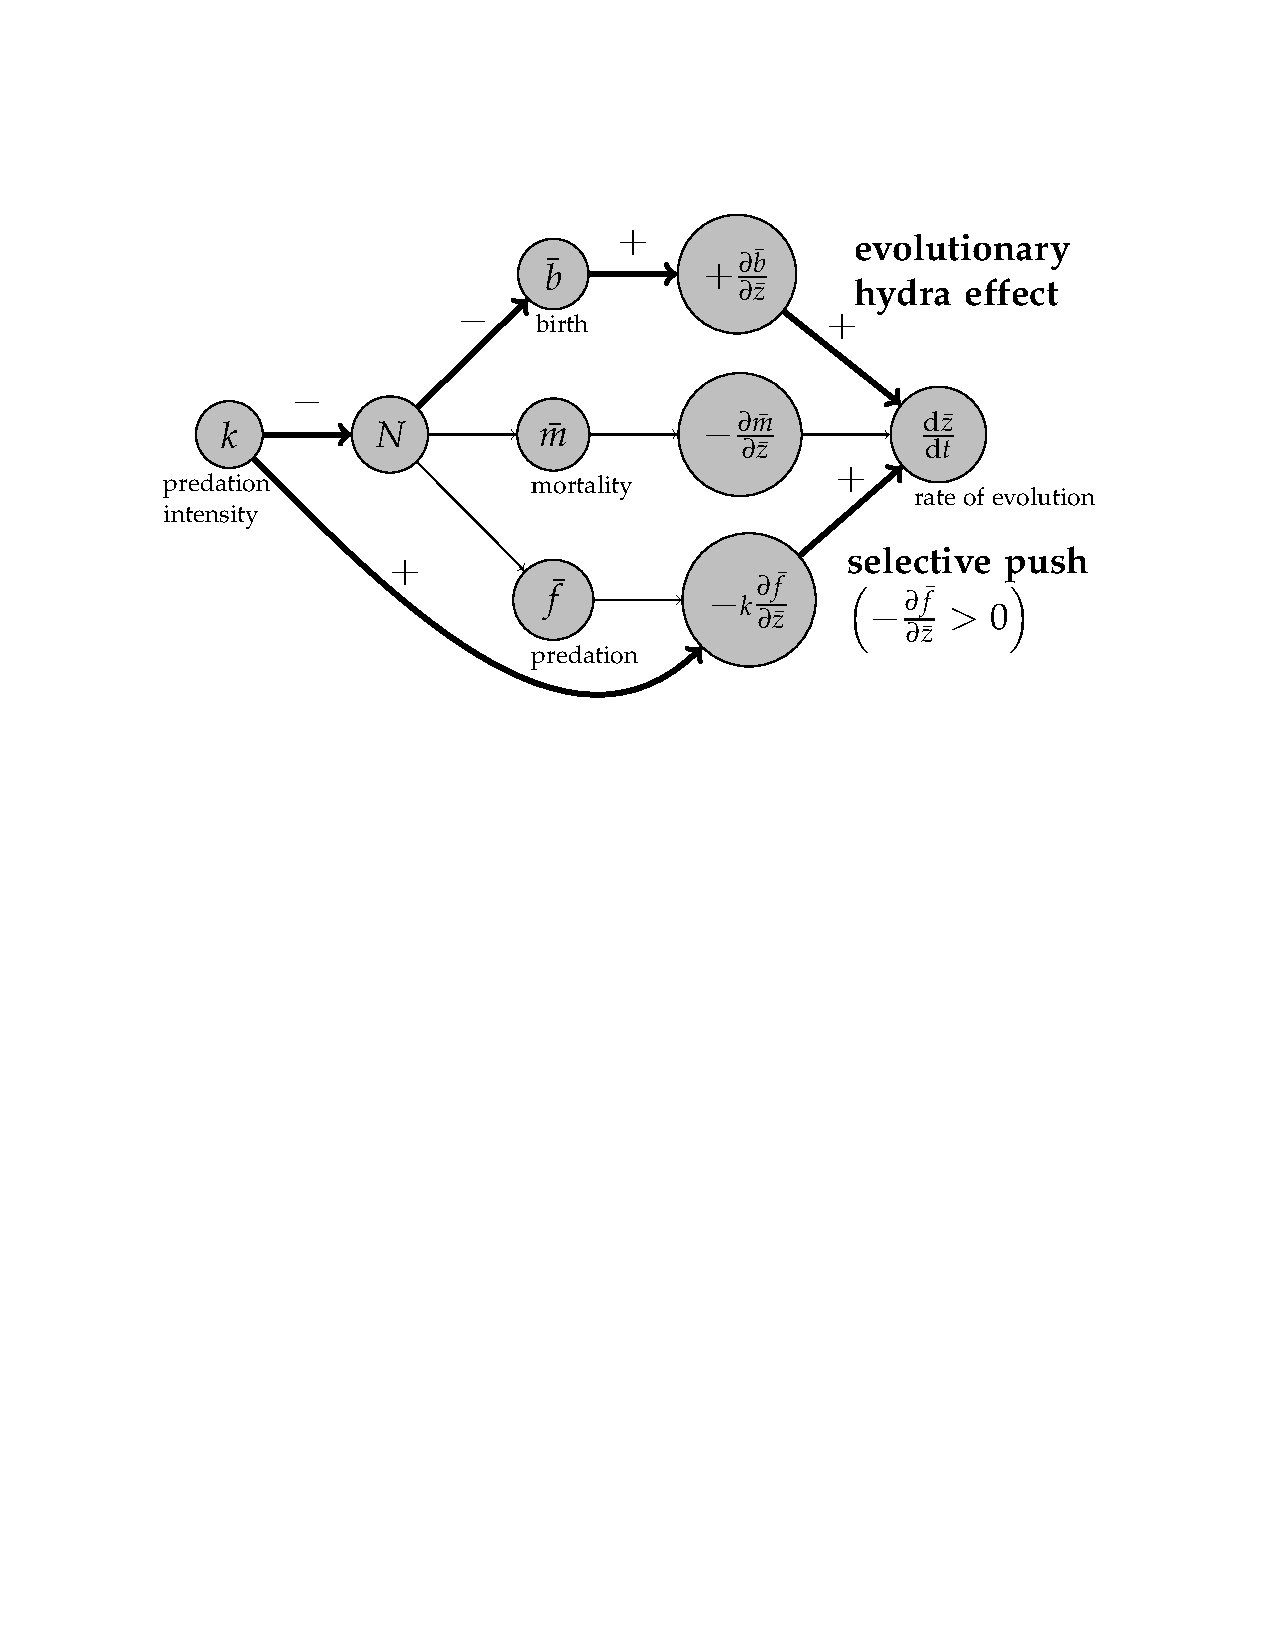
\includegraphics[width=1\linewidth, trim = 50 450 50 100, clip]{Figure1.pdf}
\caption{
Pathways by which predation intensity, $k$, can affect the rate of prey evolution, $\mathrm{d}\bar{z}/\mathrm{d}t$.
Bold lines show our two examples: the evolutionary hydra effect (top) and the selective push (bottom).
Positive and negative symbols give the sign of the partial derivative of the right variable with respect to the left variable in our examples (e.g., the negative symbol between $k$ and $N$ indicates that prey density, $N$, declines with increasing predation intensity, $\partial N/\partial k < 0$).
Increasing predation intensity increases the rate of prey evolution (towards larger trait values) via a specific pathway when the product of the signs along that pathway is positive.
}
\label{Diagram}
\end{figure}
%%%%%%%%%%%%%%%%%%%%%%%%%%%%%%%%%%%%%%%%%%%%%%%%

%%%%%%%%%%%%%%%%%%%%%%%%%%%%%%%%%%%%%%%%%%%%%%%%
\begin{figure}[!h]
\centering
%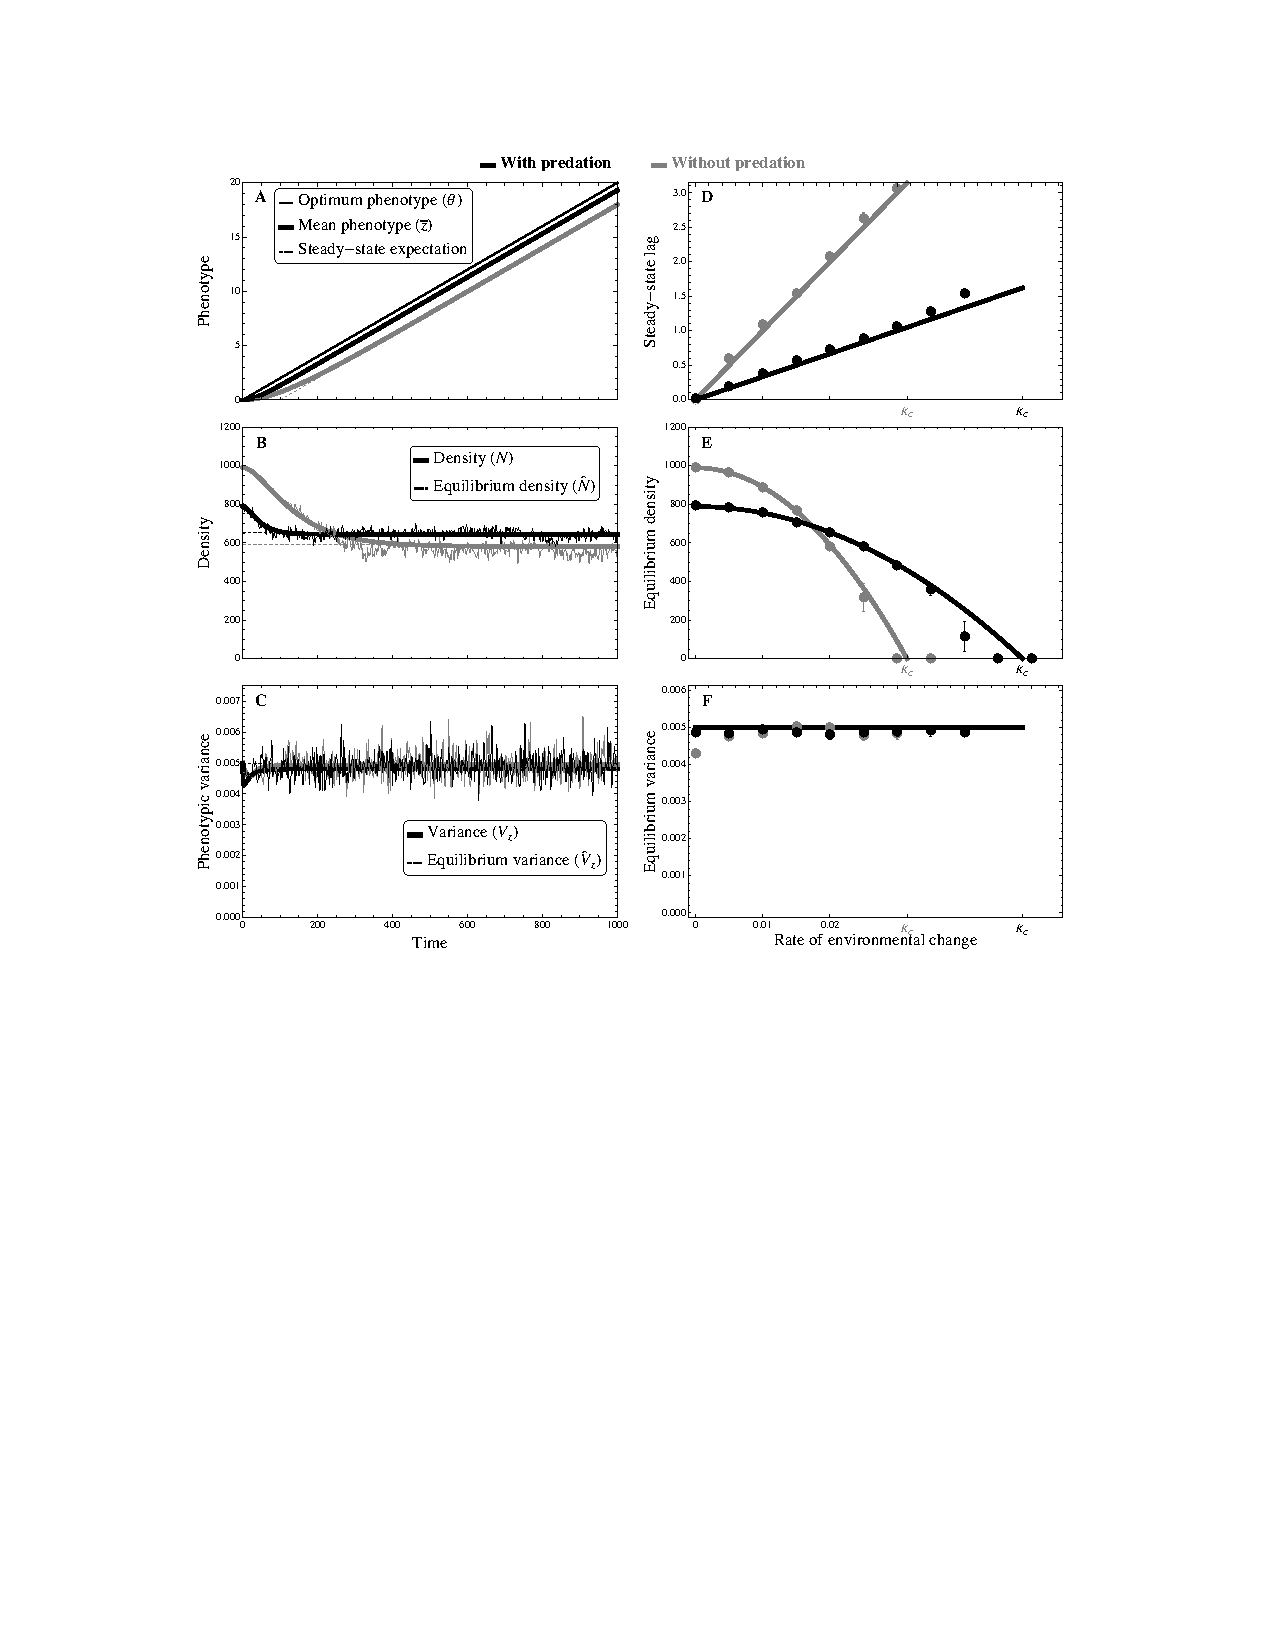
\includegraphics[width=\linewidth, trim = 75 325 75 50, clip]{Figure2.pdf}
\caption{
The selective push.
(\textbf{A,B,C}) Temporal dynamics of mean prey phenotype, population density, and phenotypic variance when $\delta = 0.02$.
\textit{Dashed} curves are analytical solutions for equilibrium values (supplementary \texttt{Mathematica} file). 
\textit{Thick} curves are numerical solutions (supplementary \texttt{Mathematica} file). 
\textit{Thin} curves are results from one simulation (obscured by thick curves in A; Online Appendix A). 
(\textbf{D,E,F}) Equilibrium dynamics of steady-state phenotypic lag, population density, and phenotypic variance as functions of $\delta$.
Curves give analytical results (supplementary \texttt{Mathematica} file). 
The dots give simulation results (mean $\pm$ 1.96 SE of 10 replicates; Online Appendix A).
Parameters: $b_{max}=0.01$, $R_{tot}=1000$, $m_{min}=0.1$, $\gamma=1$, $\gamma_k = 1$, $\alpha^2=0.05$, $k = 0$ (\textit{gray}), $k=2$ (\textit{black}).
}
\label{SelectivePush}
\end{figure}
%%%%%%%%%%%%%%%%%%%%%%%%%%%%%%%%%%%%%%%%%%%%%%%%

%%%%%%%%%%%%%%%%%%%%%%%%%%%%%%%%%%%%%%%%%%%%%%%%
\begin{figure}[!h]
\centering
%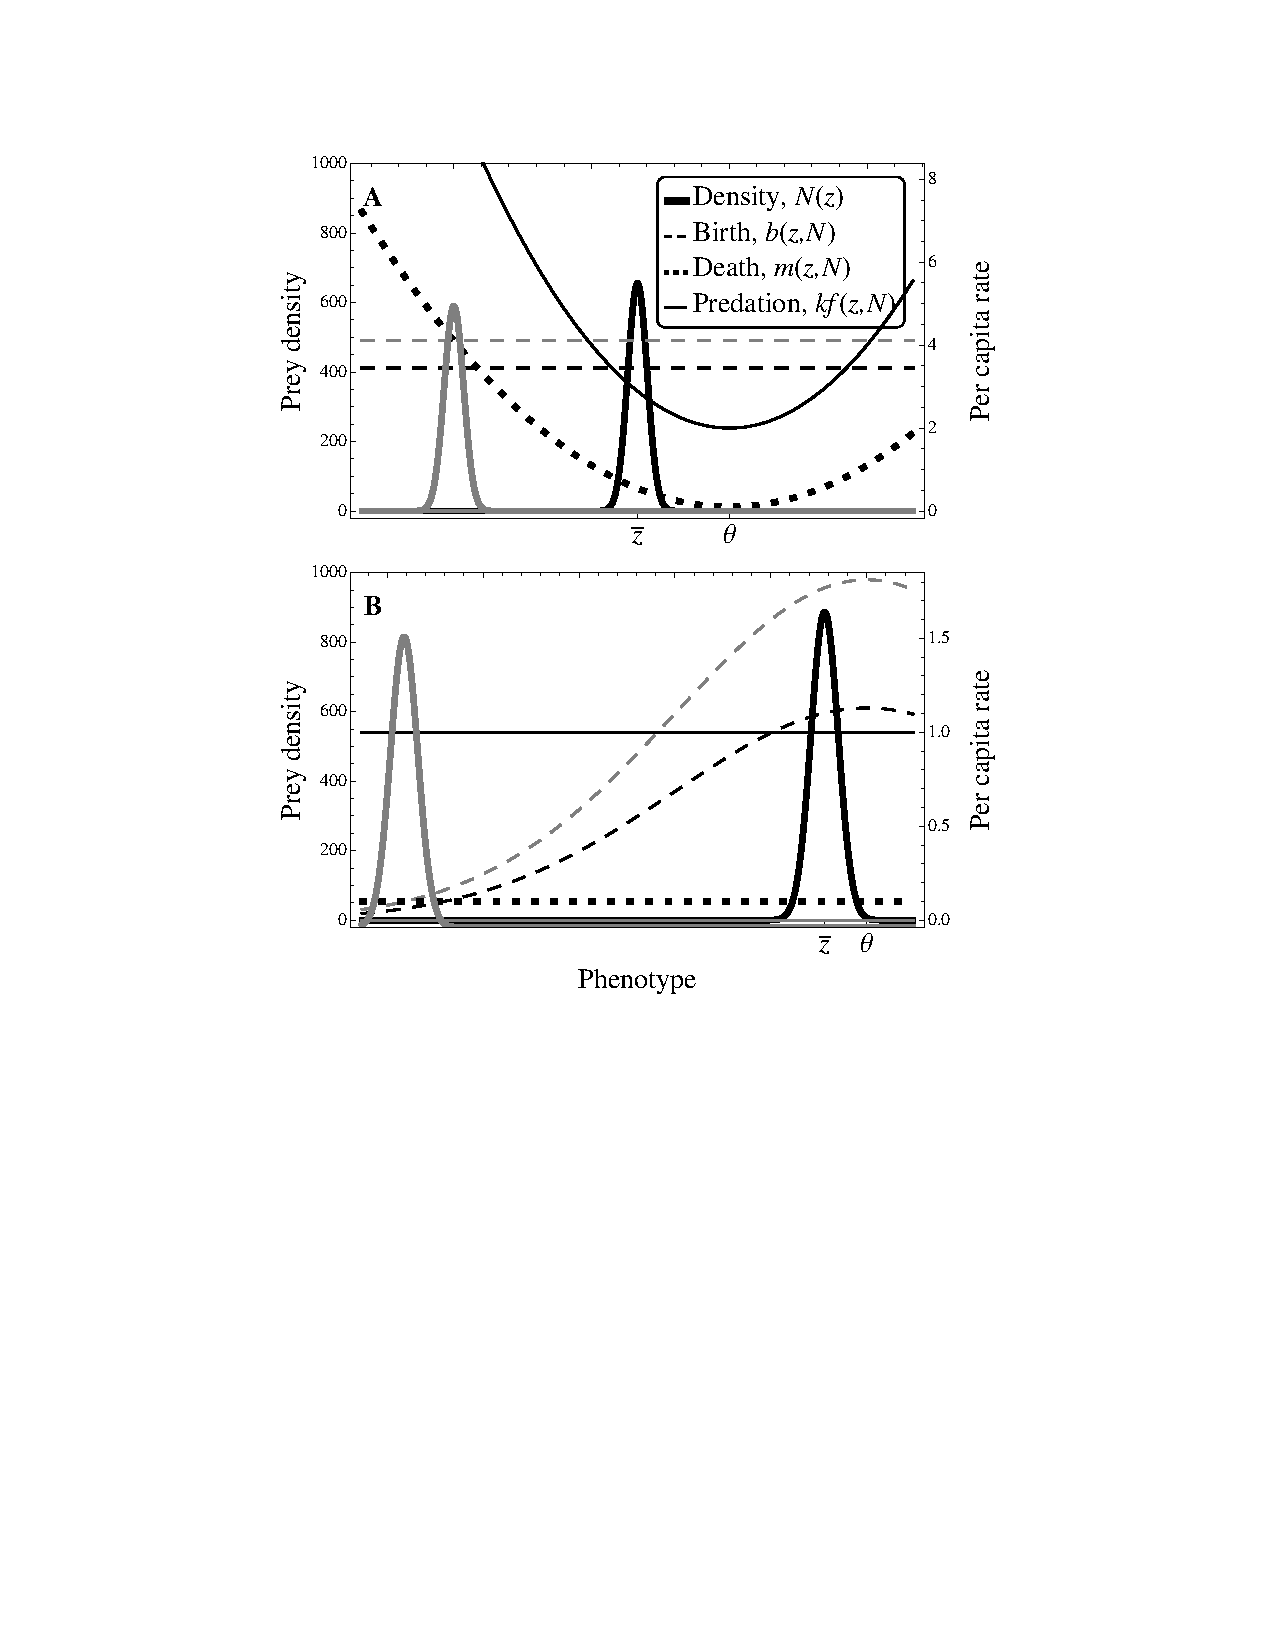
\includegraphics[width=\linewidth, trim = 75 300 75 50, clip]{Figure3.pdf}
\caption{
Graphical depiction of selective pressures in our two generalist predator examples with (\textit{black}) and without (\textit{gray}) predation.
(\textbf{A}) The selective push at the equilibrium shown in Figure \ref{SelectivePush}A-C.
(\textbf{B}) The evolutionary hydra effect at the equilibrium shown in Figure \ref{HydraEffect}A-C.
In \textbf{A} the per capita birth rate is higher in the absence of predation (\textit{grey}) because the population is further from the optimum and hence experiences more deaths, freeing up resources that increase the birth rate.
}
\label{Lande}
\end{figure}
%%%%%%%%%%%%%%%%%%%%%%%%%%%%%%%%%%%%%%%%%%%%%%%%

%%%%%%%%%%%%%%%%%%%%%%%%%%%%%%%%%%%%%%%%%%%%%%%%
\begin{figure}[!h]
\centering
%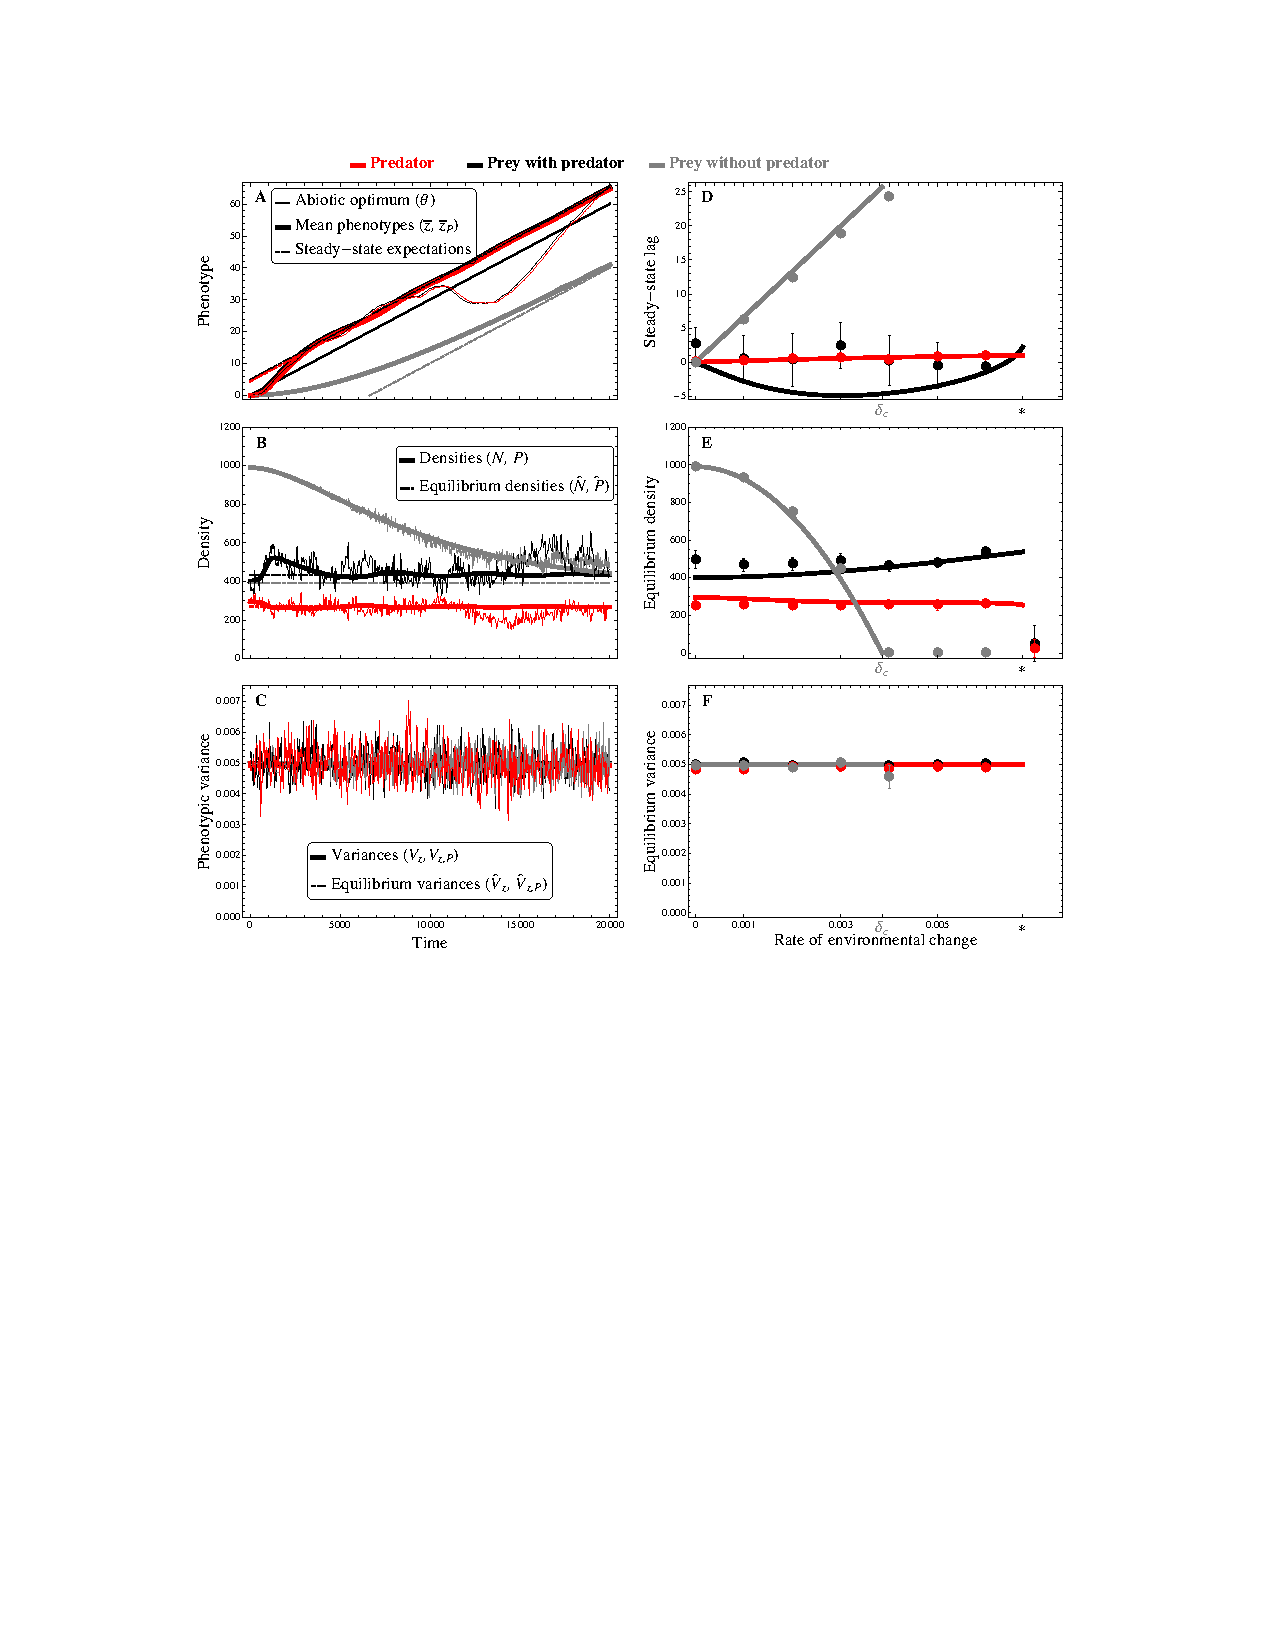
\includegraphics[width=\linewidth, trim = 75 325 75 50, clip]{Figure5.pdf}
\caption{
The evolutionary hydra effect.
(\textbf{A,B,C}) Temporal dynamics of mean prey phenotype, population density, and phenotypic variance when $\delta = 0.0006$.
\textit{Dashed} curves are analytical solutions for equilibrium values (supplementary \texttt{Mathematica} file). 
\textit{Thick} curves are numerical solutions (supplementary \texttt{Mathematica} file). 
\textit{Thin} curves are results from one simulation (obscured by thick curves in A and B; Online Appendix A). 
(\textbf{D,E,F}) Equilibrium dynamics of steady-state phenotypic lag, population density, and phenotypic variance as functions of $\delta$.
Curves give analytical results (supplementary \texttt{Mathematica} file). 
The dots give simulation results (mean $\pm$ 1.96 SE of 10 replicates; Online Appendix A).
Parameters: $b_{max}=0.01$, $m=0.1$, $R_{tot}=1000$, $\gamma=1$, $\alpha^2=0.05$, $k = 0$ (\textit{gray}), $k=1$ (\textit{black}).
}
\label{HydraEffect}
\end{figure}
%%%%%%%%%%%%%%%%%%%%%%%%%%%%%%%%%%%%%%%%%%%%%%%%

%%%%%%%%%%%%%%%%%%%%%%%%%%%%%%%%%%%%%%%%%%%%%%%%
\begin{figure}[!h]
\centering
%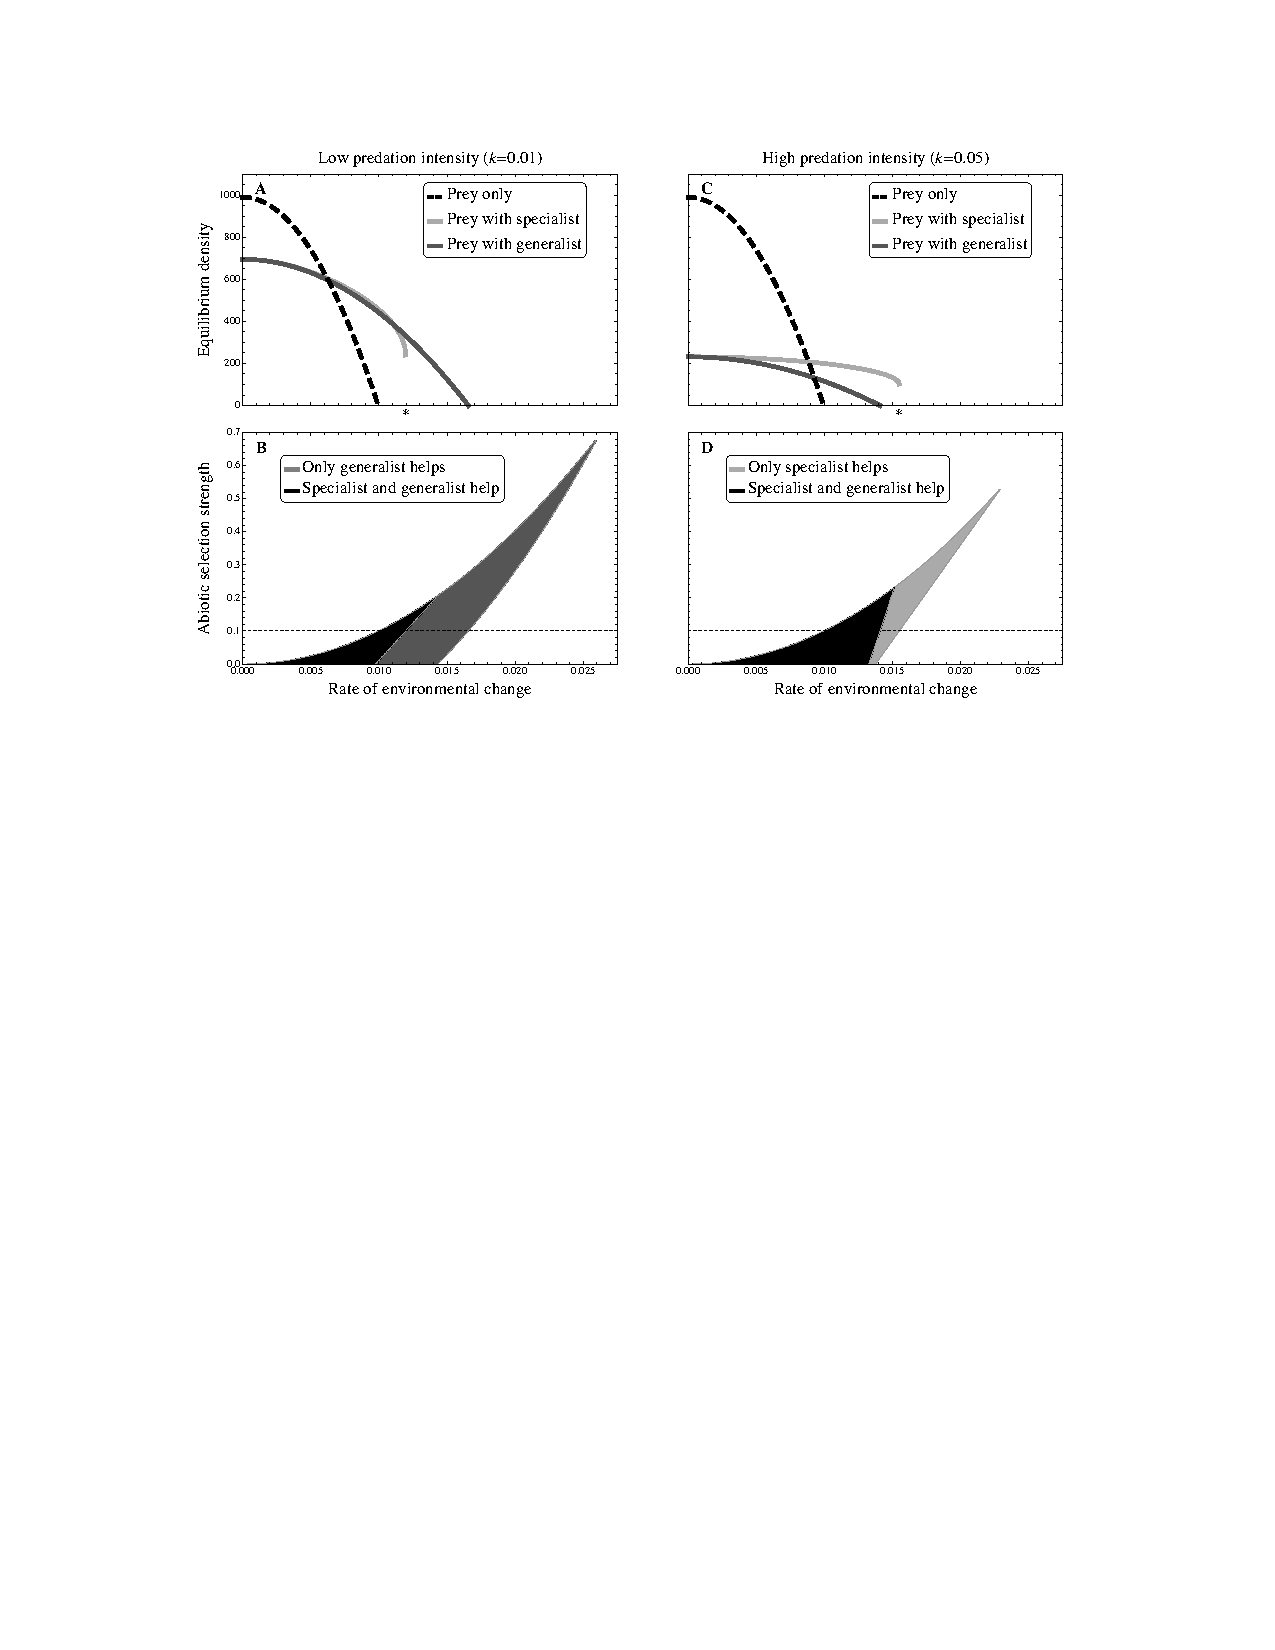
\includegraphics[width=\linewidth, trim = 75 325 75 50, clip]{Figure6.pdf}
\caption{
Coevolution between the prey (\textit{black}) and a specialist predator (\textit{red}).
(\textbf{A,B,C}) Temporal dynamics of mean prey and predator phenotypes, population densities, and phenotypic variances when $\delta = 0.003$.
\textit{Dashed} curves are analytical solutions for equilibrium values (supplementary \texttt{Mathematica} file). 
\textit{Thick} curves are numerical solutions (supplementary \texttt{Mathematica} file). 
\textit{Thin} curves are results from one simulation (\textit{gray} obscured by thick curve in A; Online Appendix A). 
(\textbf{D,E,F}) Equilibrium dynamics of steady-state phenotypic lags, population densities, and phenotypic variances as functions of $\delta$.
Curves give analytical results (supplementary \texttt{Mathematica} file).  
The dots give simulation results (mean $\pm$ 1.96 SE of 10 replicates; Online Appendix A).
Asterisk (*) denotes rate of environmental change where coevolving prey and predator equilibrium densities become complex values.
Parameters: $b=0.01$, $m_{min}=0.1$, $R_{tot}=1000$, $\gamma=0.03$, $\gamma_k=0.5$, $e=1$, $m_P=4$, $\alpha^2=0.05$, $\alpha_P^2=0.05$, $k = 0$ (\textit{gray}), $k=0.01$ (\textit{black} and \textit{red}).
}
\label{Specialist}
\end{figure}
%%%%%%%%%%%%%%%%%%%%%%%%%%%%%%%%%%%%%%%%%%%%%%%%

%%%%%%%%%%%%%%%%%%%%%%%%%%%%%%%%%%%%%%%%%%%%%%%%
\begin{figure}[!h]
\centering
%\includegraphics[width=0.45\linewidth]{IMAGES/SpecialistVsGeneralistPushLowDensity}
%\includegraphics[width=0.45\linewidth]{IMAGES/SpecialistVsGeneralistPushHighDensity}\\
%\includegraphics[width=0.45\linewidth]{IMAGES/SpecialistVsGeneralistPushLowRegion}
%\includegraphics[width=0.45\linewidth]{IMAGES/SpecialistVsGeneralistPushHighRegion}
\caption{
Prey persistence with a specialist vs.\ a generalist predator. 
Shown here is the case of a non-coevolving specialist predator that causes a selective push by predating maladapted prey  [replacing $f(z,z_P,P)$ in coevolving case with $f(z,P) = k \left[1 + \gamma_k (\theta - z)^2 \right]P$; see supplementary \texttt{Mathematica} file for details and other cases].
\textbf{(A,B)} With low predation intensity the specialist predator becomes rare and does not sufficiently push the prey at higher rates of environmental change.
\textbf{(C,D)} With high predation intensity the generalist predator exerts too high a demographic cost, while the specialist becomes rare when the prey are rare and can help the prey persist.
\textbf{(A,C)} Equilibrium prey densities across rates of environmental change with $\gamma=0.1$. \textbf{(B,D)} Parameter regions where predators help prey persist (dashed line corresponds to the $\gamma$ used in \textbf{A} and \textbf{C}).
Asterisks (*) indicate the rate of environmental change where the specialist predator and prey equilibrium population sizes simultaneously become complex values.
Parameter values: $b_{max}=0.01$, $m_{min}=0.1$, $R_{tot}=1000$, $e=0.25$, $m_P=1$, $\gamma_k=0.1$, $\alpha=0.05$.
}
\label{GenVsSpec}
\end{figure}
%%%%%%%%%%%%%%%%%%%%%%%%%%%%%%%%%%%%%%%%%%%%%%%%

\end{document}
